\subsection{Индустрия электронного светового оборудования}
\label{sec:subject:industry}

Электронное световое оборудование~--- это последовательность из сопряженных световых элементов, например светодиодов, под управлением какого-либо электронного устройства.

Начиная с конца 19-го века, когда русский электротехник Павел Николаевич Яблочков изобрел первую электрическую лампочку, и по сегодняшний день, индустрия электронного светового оборудования постоянно увеличивается в размерах. Разнообразие товаров растет, на рынке присутствует большой спрос, но и такая же большая конкуренция. Множество компаний получают контракты на освещение больших архитектурных сооружений, поставку светового оборудования для проведения различных музыкальных концертов (светомузыка) и так далее. Сама индустрия дистрибуции электронного светового оборудования ориентируется как на рынок физических лиц (украшения на елку, комнатное освещение, внешние украшения для дома), так и на юридических лиц (внешнее и внутренне освещение офисов, светомузыка, световые скульптуры). 

Рынок домашнего освещения становится все более и более популярным, особенно зарубежом. В США и Европе различные украшения на дом в Рождество очень популярны. В нашей стране схожее тоже можно наблюдать в Рождество и Новый год, но там масштабы и разнообразия продуктов куда шире. Люди тратят много денег, чтобы приобрести целые световые комплексы, позволяющие им уникально украсить свой дом и отличаться от соседей (Рисунок~\ref{fig:subject:industry:example}).

~
\begin{figure}[H]
\centering
	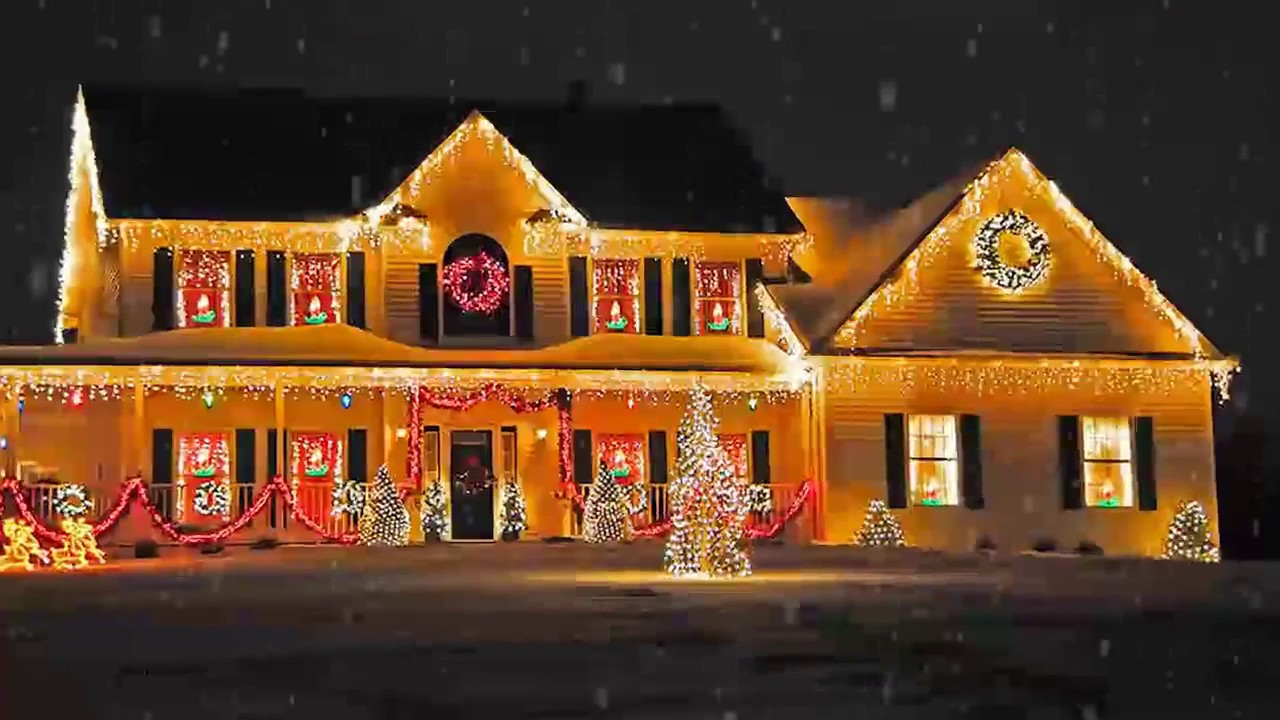
\includegraphics[scale=0.35]{figures/home_lightings.jpg}
	\caption{Пример внешнего домового освещения}
	\label{fig:subject:industry:example}
\end{figure}

Даже на фоне мирового финансового кризиса, а возможно, именно благодаря ему спрос на светодиодные источники света демонстрирует устойчивый рост по всему миру. Если еще 2–3 года назад светодиоды использовались преимущественно для вторичной декоративной подсветки, то в настоящее время технологии производства достигли того уровня, когда становится возможным их широкое применение и для функционального общего освещения.

Прогресс рынка общего освещения обусловлен двумя основными факторами. Первый — стремительный рост инвестиций в строительство в развивающихся странах. Второй — все большее внедрение дорогих технологий в освещение, включая светодиоды, что естественным образом повышает среднюю стоимость готовых осветительных приборов. Постоянно растет и рынок автомобильного освещения. В 2011 году его оборот оценивался примерно в 14 млрд евро, что составляет 20\% рынка освещения.

Так как рынок постоянно растет, сами товары совершенствуются и усложняются, то встает вопрос об управлении этими вещами. Контроллеров с маленькими дисплеями, либо просто кнопок переключения между анимациями теперь не хватает. Покупателям нужно куда больше функционала, плюс к тому, хорошо было бы иметь возможность постоянной поддержки системы управления, будь то ``патчи'' с исправлениями ошибок, либо добавление нового функционала. Для этого отлично подойдут устройства, которые и так у нас постоянно под рукой~--- мобильные телефоны. Сама же технология управления различными техническими устройствами с помощью мобильного телефона уже обзавелась названием ``Интернет вещей'' (англ. Internet of Things) или же коротко~-- IoT.